





\section{Relativistic Kinematics}
\subsection{Laboratory vs Center-of-mass frames}
A typical collision is a two-to-many reaction like:
\begin{equation}
\underbrace{A}_{\rm projectile} + \underbrace{B}_{\rm target} \rightarrow C_1 + C_2 + C_3 + \ldots,
\end{equation}

In \emph{laboratory frame}, the target is at rest, so,
\begin{equation}
	\mathbf{p}_B^{\rm lab} = \vec{0} \implies p_{B}^{\rm lab} = (m_B, 0, 0, 0),
\end{equation}

In \emph{center-of-mass} frame, the sum of three-momentum vectors vanish in the initial and final states
\begin{equation}
	\mathbf{p}_A^{\rm cm} + \mathbf{p}_B^{\rm cm} =\sum_i \mathbf{p}_{C, i}^{\rm cm} = \vec{0},
\end{equation}

Using Lorentz invariance of the Mandelstam variable \(s \equiv (p_A + p_B)_\mu(p_A + p_B)^\mu\):
\begin{align}
	s &= (E^{\rm lab}_A + m_B)^2 - |\mathbf{p}^{\rm lab}_A|^2 = (E^{\rm cm}_A + E^{\rm cm}_B)^2 \notag \\
	\implies s &= m_A^2 + m_B^2  + 2m_BE^{\rm lab}_A = (E^{\rm cm})^2 
\end{align}

As relativistic energies (\(\mathcal{O}(10^{2-3} \mathrm{GeV})\)) are much higher than reactant masses \(\mathcal{O}(1-10 \mathrm{GeV})\), 

\begin{equation}
	\sqrt{s} = E^{\rm cm} \approx \sqrt{2m_BE^{\rm lab}_A}
\end{equation}
As the center-of-mass energy that produces new particles increases only as \(\sqrt{E^{\rm lab}}\) , making any gain in particle production more expensive at relativistic energies. Thus modern colliders usually operate in center-of-mass frames.

\subsection{Coordinate system}
Considering the non-linear addition of velocities in relativistic mechanics,

\begin{equation}
	\beta = \frac{\beta_1 + \beta_2}{1 + \beta_1\beta_2},
\end{equation}

Considering the transformation \(y = \tanh^{-1}\beta\), 
\begin{align}
	\tanh^{-1}\beta_1 + \tanh^{-1}\beta_2 &= \tanh^{-1}  \frac{\beta_1 + \beta_2}{1 + \beta_1\beta_2} = \tanh^{-1}\beta\notag\\
	\implies y_1 + y_2 &= y
\end{align}

The addition is linear again.  We call this transformed velocity \emph{rapidity}, given by:
\begin{equation}
	y = \tanh^{-1}\beta = \frac{1}{2} \ln \frac{1 + \beta}{1 - \beta}  = \frac{1}{2} \ln \frac{E + p_z}{E - p_z}
	\label{eq:rapy}
\end{equation}

Rapidity can grow without bound, and at small velocities, \(y \approx \beta\), making it a relativistic analogue of velocity.  Since it transforms linearly under Lorentz boosts, rapidity distribution of particles retain their shapes. For relativistic energies, \(E \approx p\) , making \ref{eq:rapy},
\begin{equation}
	y \approx  \frac{1}{2} \ln \frac{p + p_z}{p - p_z} = -\ln\left(\tan\frac{\theta}{2}\right) = \eta
\end{equation}
\(\eta\) is called the \emph{pseudo-rapidity}, the massless limit of rapidity. As shown in \ref{fig:etavstheta}, pseudo-rapidity can be directly determined form particle production angle \(\theta\) measured with respect to the beam axis. 
\begin{figure}[htbp]
	\centering
	\begin{tikzpicture}[scale=3]
		%\message{^^JPseudorapidity including negative side}
		\pgfkeys{
			/pgf/fpu/output format=fixed, % fpu floating-point format
			/pgf/number format/precision=2 % two decimals
		}
		\def\R{1.2} % radius/length of lines
		\node[scale=1,below left=1] at (0,\R) {$y$}; % y axis
		\node[scale=1,below left=1] at (\R,0) {$z$}; % z axis
		\coordinate (O) at (0,0); % origin
		\foreach \t in {180,170,150,135,120,90,60,45,30,10,0}{ % loop over theta
				\ifnum \t = 0
					\def\e{+\infty} % infinity symbol
				\else \ifnum \t = 180
						\def\e{-\infty} % infinity symbol
					\else
						\pgfkeys{/pgf/fpu=true} % increase floating-point precision in computation
						\pgfmathparse{-ln(tan(\t/2))} % pseudorapidity
						\pgfkeys{/pgf/fpu=false} % turn off to avoid interference with following
						\pgfmathroundtozerofill{\pgfmathresult} % round with trailing zeroes
						\pgfmathsetmacro\e{\t==90?0:\pgfmathresult} % no trailing zeroes for theta = 0
					\fi \fi
				\message{^^Jt=\t, e=\e}
				\draw[eta line] % eta lines
				(O) -- (\t:\R) coordinate(P\t) node[anchor=180+\t,black] {$\eta=\e$}
				node[theta node] {$\theta=\t^\circ$};
			}
		\draw pic["$\theta$"scale=0.8,mysmallarrow] {angle = P0--O--P10}; % arrow label	
	\end{tikzpicture}
	\label{fig:etavstheta}
	\caption{\(\eta \) vs \(\theta\) }
\end{figure}

Also considering \emph{azimuthal angle} (\(\varphi\)) and \emph{transverse-momentum} \(\left(p_{\rm T} = \sqrt{p_x^2 + p_y^2}\right)\) of the particles, which are invariant under boosts along the beam-line by design, we can use (\(p_{\rm T}, \eta, \varphi\)) as the coordinate system for the particles produced in the collision. \Fref{fig:detcoords} illustrates this coordinate system for a cylindrical collider detector. 


\begin{figure}[htbp]
	\centering
	\detectorCoordinateSystem
	\caption{The \((p_{\rm T}, \eta, \varphi)\) coordinate system, drawn for a cylindrical
		collider detector. The beam axis defines \(z\) and the interaction point (IP) sits at
		the origin. A particle of momentum \(\vec{p}\) is described by its transverse momentum
		\(\vec{p}_{\rm T}\), its azimuthal angle \(\varphi\) in the transverse plane, and its
		pseudo-rapidity \(\eta\), fixed by the polar angle \(\theta\) with respect to the beam.}
	\label{fig:detcoords}
\end{figure}

%\section{Dijet events}
%In dijet events, two incoming partons, one each from the incoming nuclei scatter off each other and produce two final state partons, which are observed as jets. The two partons are back-to-back and have equal momenta in the processes center of mass frame. A typical process,
%\begin{equation}
%	\mathrm{parton}_i(p_1) + \mathrm{parton}_j(p_2) \rightarrow \mathrm{parton}_k(p_3) + \mathrm{parton}_l(p_4)
%\end{equation}
%Has parton cross-section:
%
%\begin{equation}
%	\frac{E_3E_4d^6\hat{\sigma}}{d^3p_3d^3p_4} = \frac{1}{2\hat{s}}\frac{1}{16\pi^2}\overline{\sum}|\mathcal{M}|^2\delta^4(p_1 + p_2 - p_3 - p_4)
%	\label{eq:partonxsec}
%\end{equation}
%
%Where, \(\overline{\sum}\)  denotes  the average and sum over the spins and colors of initial and final partons \(\{i, j, k, l\}\) and \(\hat{s} = (p_1+p_2)^2\). To get the dijet cross-section, we insert the parton cross-section from Eq. \ref{eq:partonxsec} into  Eq. \ref{eq:factorization}. Assuming the incoming partons are massless and collinear with the beams, \(p_1 = \frac{1}{2}x_1\sqrt{s}(1, 0, 0, 1)\) and \(p_2 = \frac{1}{2}x_2\sqrt{s}(1, 0, 0, -1)\), so that \(\hat{s} = x_1x_2s\),
%
%\begin{align*}
%	\frac{E_3E_4d^6\sigma}{d^3p_3d^3p_4} & = \frac{1}{2s}\frac{1}{16\pi^2} \sum_{\{i,j,k,l\}\subset q\bigcup\bar{q}\bigcup g} \frac{1}{1 + \delta_{kl}} \int dx_1dx_2 \frac{f_i(x_1, \mu^2)}{x_1} \frac{f_j(x_2, \mu^2)}{x_2} \\
%	& \qquad \times\, \overline{\sum}|\mathcal{M}(ij\rightarrow kl)|^2\delta^4(p_1 + p_2 - p_3 - p_4) 
%\end{align*}
%Where \(q\bigcup\bar{q}\bigcup g\) represents all the partonic states \(\{g, u, \bar{u}, d, \ldots\}\). 
%
%%	The four-momentum conserving \(\delta\)-function factorizes into a transverse part and the energy and longitudinal parts, 
%%	
%%	\begin{align*}
%	%	\delta^4(p_1 + p_2 - p_3 - p_4)                                & = \delta^2(\mathbf{p}_{T3} + \mathbf{p}_{T4})\,\delta\left(\tfrac{1}{2}\sqrt{s}(x_1 + x_2) - E_3 - E_4\right)                 \\
%	%	                                                               & \qquad \times\, \delta\left(\tfrac{1}{2}\sqrt{s}(x_1 - x_2) - p_{z3} - p_{z4}\right) \\
%	%	                                                               & = \frac{2}{s}\delta^2(\mathbf{p}_{T3} + \mathbf{p}_{T4})\,\delta\left(x_1 - \tfrac{1}{2}x_T(e^{y_3} + e^{y_4})\right)         \\
%	%	                                                               & \qquad \times\, \delta\left(x_2 - \tfrac{1}{2}x_T(e^{-y_3} + e^{-y_4})\right)
%	%\end{align*}
%	%
%	%Where, \(x_T \equiv 2p_T/\sqrt{s}\) and \(p_T \equiv p_{T, 3} = p_{T, 4}\),
%	%
%	%\begin{equation}
%	%	\frac{d^3\sigma}{dy_3dy_4dp_T^2} = \frac{1}{16\pi s^2}\sum_{\{i,j,k,l\}\subset q\bigcup\bar{q}\bigcup g} \frac{1}{1 + \delta_{kl}} \frac{f_i(x_1, \mu^2)}{x_1}\frac{f_j(x_2, \mu^2)}{x_2} \overline{\sum}|\mathcal{M}(ij\rightarrow kl)|^2
%	%\end{equation}
%	
%	Integrating Eq. \ref{eq:partonxsec} over one of the outgoing partons gives the
%	\emph{single-inclusive} parton cross-section for the other.  Writing
%	\(q \equiv p_1 + p_2 - p_3\),
%	\begin{align}
%		\frac{E_3d^3\hat{\sigma}}{d^3p_3} &= \frac{1}{2\hat{s}}\frac{1}{16\pi^2}\overline{\sum}|\mathcal{M}|^2\int\frac{d^3p_4}{E_4}\,\delta^4(p_1 + p_2 - p_3 - p_4)                              \notag                      \\
%		&=\frac{1}{2\hat{s}}\frac{1}{16\pi^2}\overline{\sum}|\mathcal{M}|^2\int\frac{d^3p_4}{E_4}\,\delta^3(\mathbf{q} - \mathbf{p}_4)\,\delta(q^0 - E_4) \notag \\
%		&= \frac{1}{2\hat{s}}\frac{1}{16\pi^2}\overline{\sum}|\mathcal{M}|^2\,\frac{\delta(q^0 - |\mathbf{q}|)}{|\mathbf{q}|}       \notag \\  
%		&= \frac{1}{2\hat{s}}\frac{1}{16\pi^2}\overline{\sum}|\mathcal{M}|^2\,2\delta(q^2)                  
%	\end{align}
%	We can represent \(q^2\) in terms of partonic Mandelstam variables \(\hat{s} = (p_1+p_2)^2\), \(\hat{t} = (p_1-p_3)^2\) and \(\hat{u} = (p_2-p_3)^2\),
%	
%	\begin{align}
%		\implies \frac{Ed^3\hat{\sigma}}{d^3p}  &= \frac{1}{2\hat{s}}\frac{1}{8\pi^2}\overline{\sum}|\mathcal{M}|^2\delta(\hat{s} + \hat{t} + \hat{u})
%	\end{align}
%	
%	Assuming perfect detector and jet algorithm, the outgoing parton's momentum is the ensuing jet's momentum.
%	\begin{align}
%		\frac{E_Jd^3\sigma}{d^3p_J}  =& \frac{1}{16\pi^2 s}\sum_{\{i,j,k,l\}\subset q\bigcup\bar{q}\bigcup g} \frac{1}{1 + \delta_{kl}}\int_{0}^{1} \frac{dx_1}{x_1}\frac{dx_2}{x_2} f_i(x_1, \mu^2) f_j(x_2, \mu^2) \notag\\ &\times\overline{\sum}|\mathcal{M}(ij\rightarrow kl)|^2\delta(\hat{s} + \hat{t} + \hat{u})
%	\end{align}
%	\begin{sidewaystable}[htbp]
%		\centering
%		\setlength{\tabcolsep}{4pt}
%		\begin{tabular}{
%				>{\centering\arraybackslash}m{2.2cm}
%				>{\centering\arraybackslash}m{2.8cm}
%				>{\centering\arraybackslash}m{2.8cm}
%				>{\centering\arraybackslash}m{2.8cm}
%				>{\centering\arraybackslash}m{2.8cm}
%				>{\centering\arraybackslash}m{6.8cm}
%			}
%			\toprule
%			Process & \multicolumn{4}{c}{Diagrams} & \(\overline{\sum}|\mathcal{M}|^2/(4\pi\alpha_s)^2\) \\
%			\midrule
%			\(qq' \to qq'\)             & \diagqqpT{q'}{q}   &                  &            &          &
%			\(\dfrac{4}{9}\dfrac{\hat{s}^2+\hat{u}^2}{\hat{t}^2}\)                                                   \\
%			\(qq \to qq\)               & \diagqqpT{q}{q}    & \diagqqU{q}      &            &          &
%			\(\dfrac{4}{9}\left(\dfrac{\hat{s}^2+\hat{u}^2}{\hat{t}^2}+\dfrac{\hat{s}^2+\hat{t}^2}{\hat{u}^2}\right)
%			-\dfrac{8}{27}\dfrac{\hat{s}^2}{\hat{u}\hat{t}}\)                                                        \\
%			\(q\bar{q}' \to q\bar{q}'\) & \diagqqbpT{q}{q'}  &                  &            &          &
%			\(\dfrac{4}{9}\dfrac{\hat{s}^2+\hat{u}^2}{\hat{t}^2}\)                                                   \\
%			\(q\bar{q} \to q'\bar{q}'\) & \diagqqbAnn{q}{q'} &                  &            &          &
%			\(\dfrac{4}{9}\dfrac{\hat{t}^2+\hat{u}^2}{\hat{s}^2}\)                                                   \\
%			\(q\bar{q} \to q\bar{q}\)   & \diagqqbAnn{q}{q}  & \diagqqbpT{q}{q} &            &          &
%			\(\dfrac{4}{9}\left(\dfrac{\hat{s}^2+\hat{u}^2}{\hat{t}^2}+\dfrac{\hat{t}^2+\hat{u}^2}{\hat{s}^2}\right)
%			-\dfrac{8}{27}\dfrac{\hat{u}^2}{\hat{s}\hat{t}}\)                                                        \\
%			\(q\bar{q} \to gg\)         & \diagqqbS          & \diagqqbT        & \diagqqbU  &          &
%			\(\dfrac{32}{27}\dfrac{\hat{t}^2+\hat{u}^2}{\hat{t}\hat{u}}
%			-\dfrac{8}{3}\dfrac{\hat{t}^2+\hat{u}^2}{\hat{s}^2}\)                                                    \\
%			\(gg \to q\bar{q}\)         & \diagggqqS         & \diagggqqT       & \diagggqqU &          &
%			\(\dfrac{1}{6}\dfrac{\hat{t}^2+\hat{u}^2}{\hat{t}\hat{u}}
%			-\dfrac{3}{8}\dfrac{\hat{t}^2+\hat{u}^2}{\hat{s}^2}\)                                                    \\
%			\(qg \to qg\)               & \diagqgS           & \diagqgT         & \diagqgU   &          &
%			\(-\dfrac{4}{9}\dfrac{\hat{s}^2+\hat{u}^2}{\hat{s}\hat{u}}
%			+\dfrac{\hat{u}^2+\hat{s}^2}{\hat{t}^2}\)                                                                \\
%			\(gg \to gg\)               & \diagggS           & \diagggT         & \diagggU   & \diagggX &
%			\(\dfrac{9}{2}\left(3-\dfrac{\hat{t}\hat{u}}{\hat{s}^2}-\dfrac{\hat{s}\hat{u}}{\hat{t}^2}
%			-\dfrac{\hat{s}\hat{t}}{\hat{u}^2}\right)\)                                                              \\
%			\bottomrule
%		\end{tabular}
%		\caption[Leading-order diagrams and matrix elements for jet production]{%
%			The complete set of leading-order diagrams and squared matrix
%			elements for the partonic \(2\to2\) processes that produce jets, entering
%			the hard cross section \(\hat{\sigma}_{ij}\) of Fig. \ref{fig:factorization}.
%			Here \(q\) and \(q'\) denote distinct quark flavours, and \(\hat{s}\),
%			\(\hat{t}\), \(\hat{u}\) are the Mandelstam invariants of the partonic
%			subprocess.  The matrix elements are averaged over
%			initial-state and summed over final-state spins and colours, as indicated
%			by \(\overline{\sum}\), and are normalised by \(g^4 = (4\pi\alpha_s)^2\)~\cite{Ellis_Stirling_Webber_1996}.}
%		\label{tab:jetdiagrams}
%	\end{sidewaystable}

\section{Jets}
The discussions on parton shower and fragmentation show partons cleanly branching into partons and eventually giving rise to hadrons that can be traced back to the shower partons. So in principle, a \emph{jet finding algorithm} should be able to faithfully get the kinematics of the initiating parton. However, the picture is not so straightforward even at the parton level, before we have the complications from hadronization and detector level reconstruction. This ambiguity can already be seen in a clean reaction like \(e^+e^-\to q\bar{q}\). If one of the quark emits a gluon, then depending on the emission angle of the gluon, we might cluster 2 or 3 jets in the final state. So one can foresee the inherent ambiguity of jet definition for more complicated hadron-hadron collisions, led to the Snowmass Accord, which stated that, experimental and theoretical measurements had to use the same jet finding algorithm  on final state hadrons in order to be comparable. 

Even after we define a jet, another ambiguity comes from the decision of what constituents in the event must be used as inputs into the jet finding algorithm. Especially, in Au+Au collisions jet-medium interactions make that choice non-trivial. Keeping these considerations in mind, a ``good'' jet finding algorithm is:
\begin{itemize}
	\item \emph{Collinear safe}, meaning  it would find the same jet with the same \(p_\mathrm{T, jet}\) regardless of  fragmentation details
	\item \emph{Infrared safe}, meaning  it would find the same jets, even in the presence of a
	large number of soft partons
\end{itemize}

The most commonly used family of infrared and collinear safe jet algorithms, sequentially recombines constituents in an event according to the following prescription:

\begin{enumerate} 
	\item Calculate
	\begin{equation}
		d_{ij} = {\mathrm {min}}(p_{T,i}^{2p},p_{T,j}^{2p})\frac{(\eta_i-\eta_j)^2+(\phi_i-\phi_j)^2}{R^2}
	\end{equation}
	and 
	\begin{equation}
		d_{i} = p_{T,i}^2p
	\end{equation}
	for every pair of particles where $p_{T,i}$ and $p_{T,j}$ are the momenta of the particles, $\eta_i$ and $\eta_j$ are the pseudorapidities of the particles, and $\phi_i$ and $\phi_j$ are the azimuthal angles of the particles. \(R\) is the resolution parameter of the algorithm, which decides the angular extent of clustered jets.
	\item Find the minimum of the $d_{ij}$ and $d_{i}$.  If this minimum is a $d_{ij}$, combine these particles into one jet candidate, adding their energies and momenta, and return to the first step.  
	\item If the minimum is a $d_{i}$, this is a final state jet candidate.  Remove it from the list and return to the first step.  Iterate until no particles remain.  
\end{enumerate}

Above algorithm becomes the \(k_\mathrm{T}\) algorithm for \(p=1\), Cambridge-Aachen for \(p=0\) and the most widely used anti- \(k_\mathrm{T}\) algorithm for \(p=-1\). 

\subsection{SoftDrop}

\subsection{Background Subtraction}

\section{Heavy-Ion Collisions}
\label{sec:heavyIonCollisions}


\subsection{Centrality determination} \label{sect:CentEP}
In heavy-ion collisions, the impact parameter (\(b\)) of collisions is defined by the distance between the geometrical centers of the colliding nuclei in the plane transverse to their direction. A schematic diagram of the geometry of heavy-ion collisions is shown in Fig. \ref{fig:hictikz}. 
\begin{figure}[htbp]
	\centering
	\begin{tikzpicture}
		\def\N{85} % number of nucleons
		\def\R{1.0} % nucleus radius
		\def\Nlay{5} % number of rings/layers
		\def\xs{0.25} % horizontally scale
		\def\Rp{0.92} % length photon
		\def\D{3.7} % horizontal distance between nuclei
		\pgfmathsetmacro\H{1.30*\R} % vertical distance between nuclei
		\pgfmathsetmacro\v{0.25*\D} % length vector
		
		%\message{^^J PbPb collision with impact parameter}
		
		% NUCLEUS
		\pic[xscale=\xs] (L) at (-\D/2, \H/2) {nucleus};
		\pic[xscale=\xs] (R) at ( \D/2,-\H/2) {nucleus};
		
		% VELOCITY VECTORS
		\draw[vector] (L-0)++(2pt,0) --++ (\v,0); %node[above=2pt] {$v\approx c$};
		\draw[vector] (R-180)++(-2pt,0) --++ (-\v,0); %node[above=2pt] {$v\approx c$};
		
		% PHOTONS
		\foreach \ang in {60,90,120,-60,-90,-120}{
			\draw[photon] (L-\ang) --++ (\ang:\Rp);
			\draw[photon] (R-\ang) --++ (\ang:\Rp);
		}
		
		% MEASURES
		\draw[<->,thick]
		(R-0)++(0.3*\R,0) --++ (0,\R) node[midway,right] {$R\sim A^{1/3}\mathrm{fm}$};
		\draw[<->,thick]
		(0,-\H/2) -- (0,\H/2) node[midway,right] {$b$};
		%\node at (0.3*\D,0.7*\H) {$b > 2R$};
		
	\end{tikzpicture}
	\caption{Typical heavy-ion collision}
	\label{fig:hictikz}
\end{figure}
As the impact parameter is not measurable in experiments, the charged particle multiplicity of events can be used to define collision centrality as they reflect the initial geometry of the colliding nuclei. To obtain the geometrical quantities like the impact parameter, the number of participant nucleons (\(N_\mathrm{part}\)) and the number of binary collisions (\(N_\mathrm{coll}\)), one has to rely on model calculations which involves mapping the charged particle multiplicity from experiment to that of a simulated one. The widely used model for determining these quantities is the Glauber Monte Carlo (Glauber MC) model. In Glauber model, nucleons in a nuclei are distributed following the Wood–Saxon density distribution. The nuclei are then assigned a random impact parameter and translated to collide. The distance between the centers of nucleons of each nucleus is calculated. If this distance is found to be less than \(\sqrt{\sigma_\mathrm{inel}^\mathrm{NN}/\pi}\), where \(\sigma_\mathrm{inel}^\mathrm{NN}\) is the inelastic nucleon–nucleon cross section, the nucleons have undergone a binary collision. Nucleons that have undergone at least one binary collision are said to have participated in the reaction. This procedure is followed to obtain \(N_\mathrm{part}\), \(N_\mathrm{coll}\) event-by-event.

A class of events belonging to a given centrality (say 0\%–5\%) is obtained by the collection of events representing the fraction of the total cross-section. Glauber model can only provide the information on \(N_\mathrm{part}\), \(N_\mathrm{coll}\) and impact parameter \(b\), but for mapping with the experimental data, one has to use a combination of the Glauber model and a particle production model called the Two-Component Model. Assuming that particle production is governed by contribution from hard component (proportional to \(N_\mathrm{coll}\)) and soft component (proportional to  \(N_\mathrm{part}\)), it simulates the multiplicity distribution according to

\begin{equation}
	N_\mathrm{ch} = n_{pp}\left[xN_\mathrm{coll} + (1-x)\frac{N_\mathrm{part}}{2}\right]
\end{equation}
where the quantity \(n_{pp}\) is the multiplicity from a \(p+p\) collision of the same center-of-mass energy. \(x\) is the contribution of hard component. \(n_{pp}\) is drawn from a negative binomial distribution with parameters \(\text{NBD }(n_{pp}; \langle n_{pp}\rangle,k)\), where \( \langle n_{pp}\rangle\) is the average multiplicity in the \(p+p\) collision and \(k\) is the width of the distribution. The simulated charged multiplicity distribution is then fitted with the corresponding multiplicity distribution from the experiment. \(\langle n_{pp}\rangle\), \(k\), and \(x\) are kept as free parameters in the fitting to experimentally measured charged particle multiplicity distribution. Initial guess values for \(x\) could be set close to those determined in different experiments for faster convergence of fitting. 
\begin{figure}[h]
	\label{fig:centralityVsNch}
	\centering
	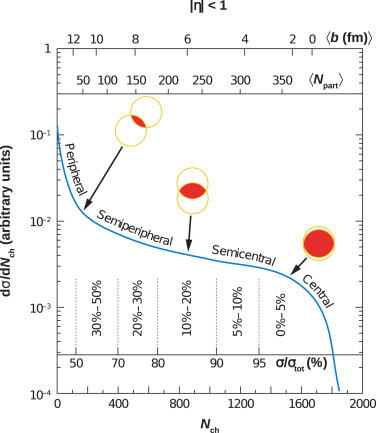
\includegraphics[width=0.6\textwidth]{figures/centrality_refmult.jpg}
	\caption{An illustration of the total inclusive charged particles multiplicity \(N_\mathrm{ch}\) and number of participant (\(N_\mathrm{part}\)) and impact parameter (\(b\)) in heavy-ion collisions}
\end{figure}
Fig.~\ref{fig:centralityVsNch} illustrates collision centrality definition in heavy-ion collisions by comparing the charge particle multiplicities with Glauber MC + Two-component model simulation. Centrality classes are classified for the simulated distribution. \(\langle N_\mathrm{part}\rangle\), \(\langle N_\mathrm{coll}\rangle\) in those centrality classes are calculated.


\subsection{Event plane reconstruction}
\begin{figure}[h]
	\centering
	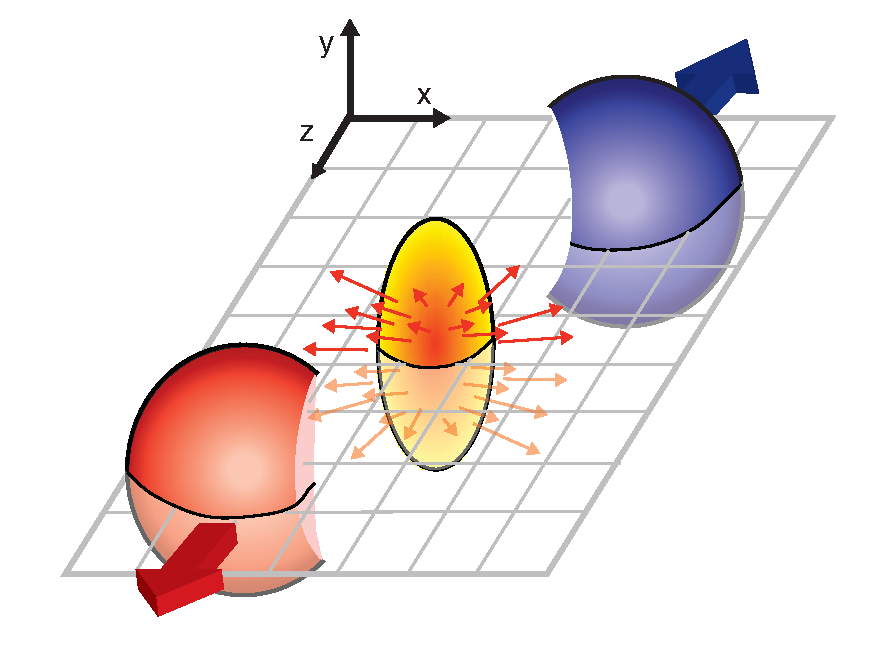
\includegraphics[width=0.4\textwidth]{figures/flow_elliptic_init_v4.pdf}
	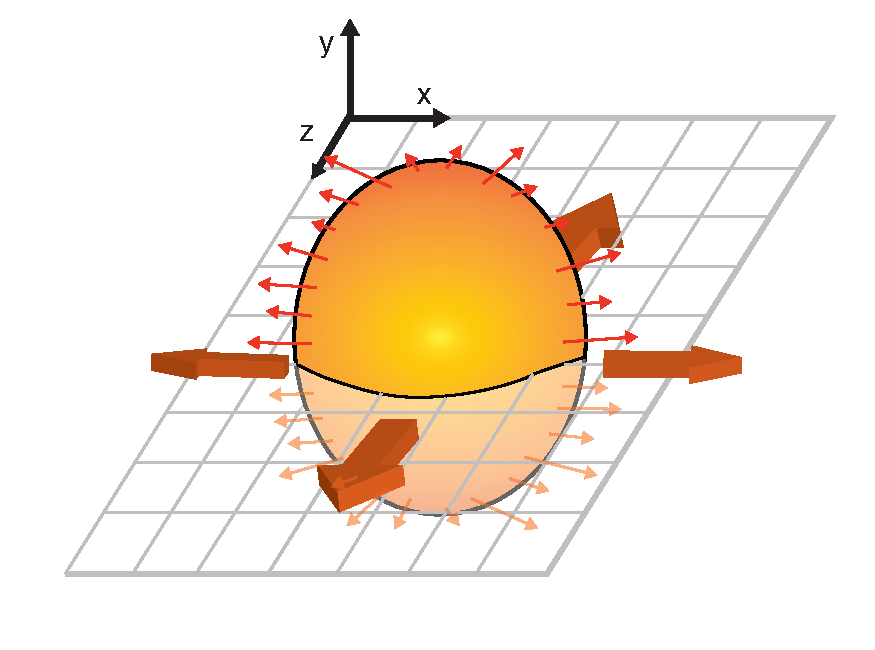
\includegraphics[width=0.4\textwidth]{figures/flow_elliptic_expd_xyz_v2.pdf}
\end{figure}
Within the overlap region, symmetry planes are generated from initial asymmetries in the nucleon distributions and can be quantified by a harmonic decomposition ~\cite{Poskanzer:1998yz}.  The reaction plane would correspond to the second-order symmetry plane $\Psi_{2, EP}$ if nucleon distributions were in their average positions and devoid of fluctuations of interactions amongst nucleons ~\cite{PhysRevC.101.064901}.  We refer in this letter to the event plane as being the experimentally reconstructed second-order symmetry plane ~\cite{Poskanzer:1998yz}.

By measuring the charged particle azimuthal distribution, the n-th order event plane can be extracted by \cite{Poskanzer:1998yz}:  

\begin{equation}
	\Psi_{n,EP} = \frac{1}{n} \arctan \left(\frac{Q_{y, n}}{Q_{x, n}} \right),
	\label{eqn:EP}
\end{equation}

Where, the weighted $Q$ vectors are given by:

\begin{align}
	Q_{x, n} = \sum_{\mathrm{tracks}} w_{\rm track} \cos (n \phi_{\rm track}) \qquad \text{\&} \qquad& Q_{y, n} = \sum_{\mathrm{tracks}} w_{\rm track} \sin (n \phi_{\rm track}).
	\label{Eqn:Qvecs}
\end{align}

\noindent where the sum is calculated for all
reconstructed charged particles (tracks) in the event, $\phi_{\rm track}$ is the track's azimuthal angle, and $w_{\rm track}$ the weight associated with the track.  Weights, $w_{\rm track}$, are optimized to calculate the event-plane vector to the best accuracy. This work uses the common approach of scaling by the track's $p_{\mathrm{T}}$ ($w_{\rm track} = p_{\rm T, track}$)~\cite{Poskanzer:1998yz}.  The event plane is calculated event-by-event, following a procedure similar to Ref.~\cite{CASTILHO2018369} using charged tracks with $0.2 < p_{\rm  T, track} < 1.0$ \GeVc measured within the TPC.  The approach is called the Modified Reaction Plane (MRP) method \cite{Agakishiev:2014ada}.  Additional details can be found in Refs.~\cite{CASTILHO2018369,Adams_2005}.
% 0.2-2.0

The impact of highly energetic jets on the calculation of the event-plane orientation is reduced by removing the particles within the pseudorapidity strip ($|\deta|<0.4$) across \dphi surrounding the leading jet.  This procedure also removes a significant portion of the away-side jet, located opposite in azimuth. 
An upper limit of 1.0 GeV/c is used in the calculation of the event plane to exclude the momentum range of particles used in correlation functions from the calculation of the event plane which is used to characterize the near-side jets. Due to finite acceptance and multiplicities, the calculated event plane has an underlying anisotropy that is corrected by applying two separate correction methods.  

%Two corrections are used to flatten the raw event plane distribution.  
First, a calibration and recentering correction procedures are applied to remove bias introduced by non-uniform acceptance of the TPC tracking system and further account for potential beam-condition effects\cite{Barrette:1997pt,PhysRevC.55.1420,Poskanzer:1998yz}.  This procedure involves recentering the weighted $Q$-vectors such that, $\langle Q_{x, n} \rangle = 0 = \langle Q_{y, n} \rangle$.  

Recentering is done by calculating a modified $Q$-vector, obtained by subtracting an event averaged $Q$-vector from each event's nominal $Q$-vector and done for 10\% centrality intervals and 4 cm $v_z$ intervals.  The recentering approach, which drastically improves the uniformity of the event plane, is however, unable to remove the higher harmonics of $\Psi_{n,EP}$ \cite{Poskanzer:1998yz}.  To help remove higher harmonics and make the event-plane angle isotropic in the lab frame \cite{Voloshin:2008dg}, a second correction step, referred to as shifting, is applied event-by-event.  This method defines a new angle:

\begin{equation}
	\Psi'_{2,EP} = \Psi_{2,EP} + \sum_n \frac{2}{n}
	(- \langle \sin (n\Psi_{2,EP}) \rangle \cos(n\Psi_{2,EP}) + \langle \cos(n\Psi_{2,EP}) \sin(n\Psi_{2,EP}) \rangle) ,
	\label{eqn:Shift}
\end{equation}

\noindent where the brackets denote an average over events.  We require the vanishing of each n-th Fourier moment up to 20th order.  Similarly to recentering, the shifting correction is done separately for 10\% centrality intervals and 4-cm $v_z$ intervals.  Additional details of the recentering and shifting corrections can be found in Refs.~\cite{Wang:2012bga,Barrette:1997pt,Poskanzer:1998yz}

The resulting azimuthal anistropy can be characterized by the Fourier decomposition of the azimuthal particle distribution with respect to the second-order event plane ~\cite{Bielcikova:2003ku,Voloshin:1994mz}:

\begin{equation}
	\frac{dN}{d(\phi - \Psi_{RP})} = \frac{N_0}{2\pi} \left( 1 + 2 \sum_{n=1}^{\infty} v_n \cos[n(\phi - \Psi_{RP})] \right),
	\label{fourier_azi_part_distr}
\end{equation}

\noindent where $N_0$ is the number of particles, $\phi$ describes the azimuthal angle of the particles, $\Psi_{RP}$ describes the azimuthal angle of the true reaction plane determined by the beam axis and the impact parameter and $v_n$ is the n-th harmonic (flow) coefficient. $\Psi_{RP}$ is not experimentally known and is replaced by the reconstructed event-plane angle.  Due to finite event multiplicity, there will be a difference between these two planes.  It is quantified by event-plane resolution, $R_n$ or $R_n\{\Psi_{2, EP}\}$ given by Eqn.~\ref{resolution}. The observed $v_n$, $v_n^{\rm obs}$ is corrected for this limited resolution by doing, $v_n = v_{n}^{\rm obs}/R_n$ \cite{Abbas:2013taa,Poskanzer:1998yz}.  Because an ideal event-plane resolution is equal to 1, for non-ideal cases, the value of the coefficients will be raised by applying the correction. Thus, $R_n$ impacts the flow-modulated background for these correlations, as described in Sect.~\ref{sect:CorrBkgd},

\begin{equation}
	R_n = R_n\{\Psi_{2, EP}\} = \langle \cos(n[\Psi_{RP} - \Psi_{2, EP}]) \rangle \qquad \text{$n$ is even}
	\label{resolution}
\end{equation}

Furthermore, individual events are divided into two random sub-events by assigning charged tracks to sub-events, ``$a$" and ``$b$". The sub-events are unique, with approximately equal multiplicities. We can write the correlation of two event planes by taking the product of two sub-events \cite{Barrette:1996rs,Poskanzer:1998yz}:

\begin{equation}
	\langle \cos(n[\Psi_{2, EP}^{a} - \Psi_{2, EP}^{b}]) \rangle = 
	\langle \cos(n[\Psi_{2, EP}^{a} - \Psi_{RP}]) \rangle
	\langle \cos(n[\Psi_{2, EP}^{b} - \Psi_{RP}]) \rangle,
	\label{resolution2sub}
\end{equation}

\noindent This allows calculation of the event-plane resolution directly from data. Since $a$ and $b$ have equal multiplicities, the resolution of each sub-event can be calculated from the correlation between the two sub-events as \cite{Poskanzer:1998yz}:

\begin{equation}
	\langle \cos(n[\Psi_{2, EP}^{a} - \Psi_{RP}]) \rangle = 
	\sqrt{\langle \cos(n[\Psi_{2, EP}^{a} - \Psi_{2, EP}^{b}]) \rangle} .
	\label{resolutionIndiv}
\end{equation}

The event-plane resolution is multiplicity dependent and calculated for separate ranges of collision centrality using the two sub-events method.  Narrower bins are calculated and then combined accordingly to match the ranges used by this analysis, by averaging the results from the narrow bins weighted by the multiplicity of each bin \cite{Voloshin:2008dg}.


\section{Signatures of QGP}
Different seminal results go here...
